\chapter{Implementation}

\section{Vision system}

\subsection{Image Processing with ORBBEC Astra Camera}
The image data is sent from the camera to the connected notebook for processing.\par
There is the ROS Master and several other individual ROS nodes running on the notebook. Some ROS nodes are involved in image processing, while others provide tools such as geometric calculations or displaying detected objects and skeletons on the RViz screen.\par
ROS nodes communicate with each other using ROS messages.\par
I used two main tools to process the camera data: the ROS Astra camera driver ros\_astra\_camera for object detection and the ORBBEC Astra SDK for skeleton detection.\par
Both tools use OpenNI as an intermediate layer to access the camera data. I couldn't run them at the same time because it led to runtime errors, so I decided to split the process into two separate phases.\par
First, the ros\_astra\_camera driver is started. Once all objects are detected, the driver stops.\par
In the second phase, data is exposed by the ORBBEC Astra SDK until both pointing gestures are confirmed and the result is sent to the robot. \par
Since gesture recognition is performed within the ROS system, additional ROS packages were needed to publish the body tracking data provided by the SDK as ROS messages.\par

\subsection{Installation}

\subsubsection{ROS Noetic}
The notebook with Ubuntu 20.04 was used, for which the recommended version of the ROS distribution is ROS Noetic. I followed the instructions from http://wiki.ros.org/noetic/Installation/Ubuntu to download and install the ROS Noetic package.\par

\subsubsection{Astra and OpenNI SDKs}
For the ORBBEC Astra camera, I needed to install the Astra SDK and the OpenNI SDK for Linux.\par
Both SDKs are available at https://www.orbbec.com/developers.\par

\subsubsection{ROS Driver for Astra camera}
I downloaded the ROS driver package\\
from https://github.com/orbbec/ros\_astra\_camera and installed the dependencies according to the instructions on http://wiki.ros.org/astra\_camera.\par
The ros\_astra\_camera package supports the ROS distributions Kinetic and Melodic. I needed to find and test multiple versions of the "ros-*-libuvc-*" libraries, as they were not released specifically for ROS Noetic.\par
This problem was already solved on the ORBBEC GitHub page, so I followed the advice and installed the missing dependencies using:\par

\begin{lstlisting}[language=bash]
  $ apt install ros-noetic-rgbd-launch libuvc-dev
\end{lstlisting}


I built the package with "catkin\_make" command and was able to run code samples that show the camera data on the screen.\par

\subsubsection{ROS Packages for Gesture Based Control}
I downloaded three ROS packages from the Shinsel Robots repository on https://github.com/shinselrobots.\par
The "pcl\_object\_detection" package allows object detection in the camera data provided by the ROS Astra driver using the Point Cloud Library.\par
The "astra\_body\_tracker" and "body\_tracker\_msgs" packages publish body tracking data from the Astra SDK as ROS messages.\par
Several environment variables have to be set to indicate the paths to the AstraSDK and OpenNI subfolders.\par
For example, if "/home/user/AstraSDK" is the folder containing the Astra SDK and "/home/user/OpenNI-Linux-x64-2.3.0.66" is the folder containing the OpenNI SDK, the setting can be made by running these commands in the terminal: \par

\begin{lstlisting}[language=bash]
  $ export ASTRA_SDK=/home/user/AstraSDK
  $ export ASTRA_ROOT=/home/user/AstraSDK
  $ export ASTRA_SDK_INCLUDE=/home/user/AstraSDK/include
  $ export ASTRA_SDK_LIB=/home/user/AstraSDK/lib
  $ export OPENNI2_INCLUDE=/home/user/OpenNI-Linux-x64-2.3.0.66
  $ export OPENNI2_REDIST=/home/user/OpenNI-Linux-x64-2.3.0.66/Redist
\end{lstlisting}

\subsection{Source Code}

\subsubsection{Catkin Workspace} 
Catkin is the official build system for ROS. Project packages that are placed in the same catkin workspace can be built all at once.\par
My catkin workspace folder contains following ROS packages, all with source code written in C++: \par

\begin{itemize}
	\item ros\_astra\_camera
    \item task\_execution
    \item rviz\_screen
    \item pcl\_object\_detection
    \item pointing\_gesture
\end{itemize}

\subsubsection{Program Overview} 
  
The main launch file is task\_execution.launch. It starts the ROS Astra driver, RViz and other ROS nodes involved in the task: task\_execution\_node, pcl\_object\_detection\_node and pointing\_gesture\_node.\par
The task\_execution\_node subscribes to ROS messages\\
"pcl\_object\_detection/detected\_objects" and "body\_tracker/intersection".\\
The "pcl\_object\_detection/detected\_objects" message contains an array of coordinates of the detected objects, the "body\_tracker/intersection" message contains the coordinates of the intersection of the pointing ray and the floor.\par
When the intersection message is received for the first time, the nearest object is calculated. The object is represented by its index in the detected object array, which is then published in the "task\_execution/pointed\_object\_index" message.\par
The second received intersection message indicates the target location.
Once received, the node creates a result file and writes the coordinates of all detected objects, the coordinates of the target location and the index of the selected object.\par
Then the node connects to the robot's computer using SSH, transfers the file there and remotely starts the robot's main program.\par


\subsubsection{Object Detection with Point Cloud Library}
Point Cloud Library (PCL) was used as a tool for processing the image data.\par
The pcl\_object\_detection package allows the detection of objects on a flat surface and depends on two PCL packages: pcl\_ros and pcl\_conversions.\par
The pcl\_ros package bridges ROS systems and 3D applications that work with point clouds. It extends the ROS C++ Client Library to support messages with native PCL data types.\par
Conversions between PCL data types and ROS message types are provided by the pcl\_conversions package.\par
The pcl\_object\_detection\_node subscribes to the topic \\"/astra\_camera/depth/points", which is published by the ROS Astra camera driver. The received messages represent a point cloud with no color information.\par

\begin{figure}[h]
    \centering
    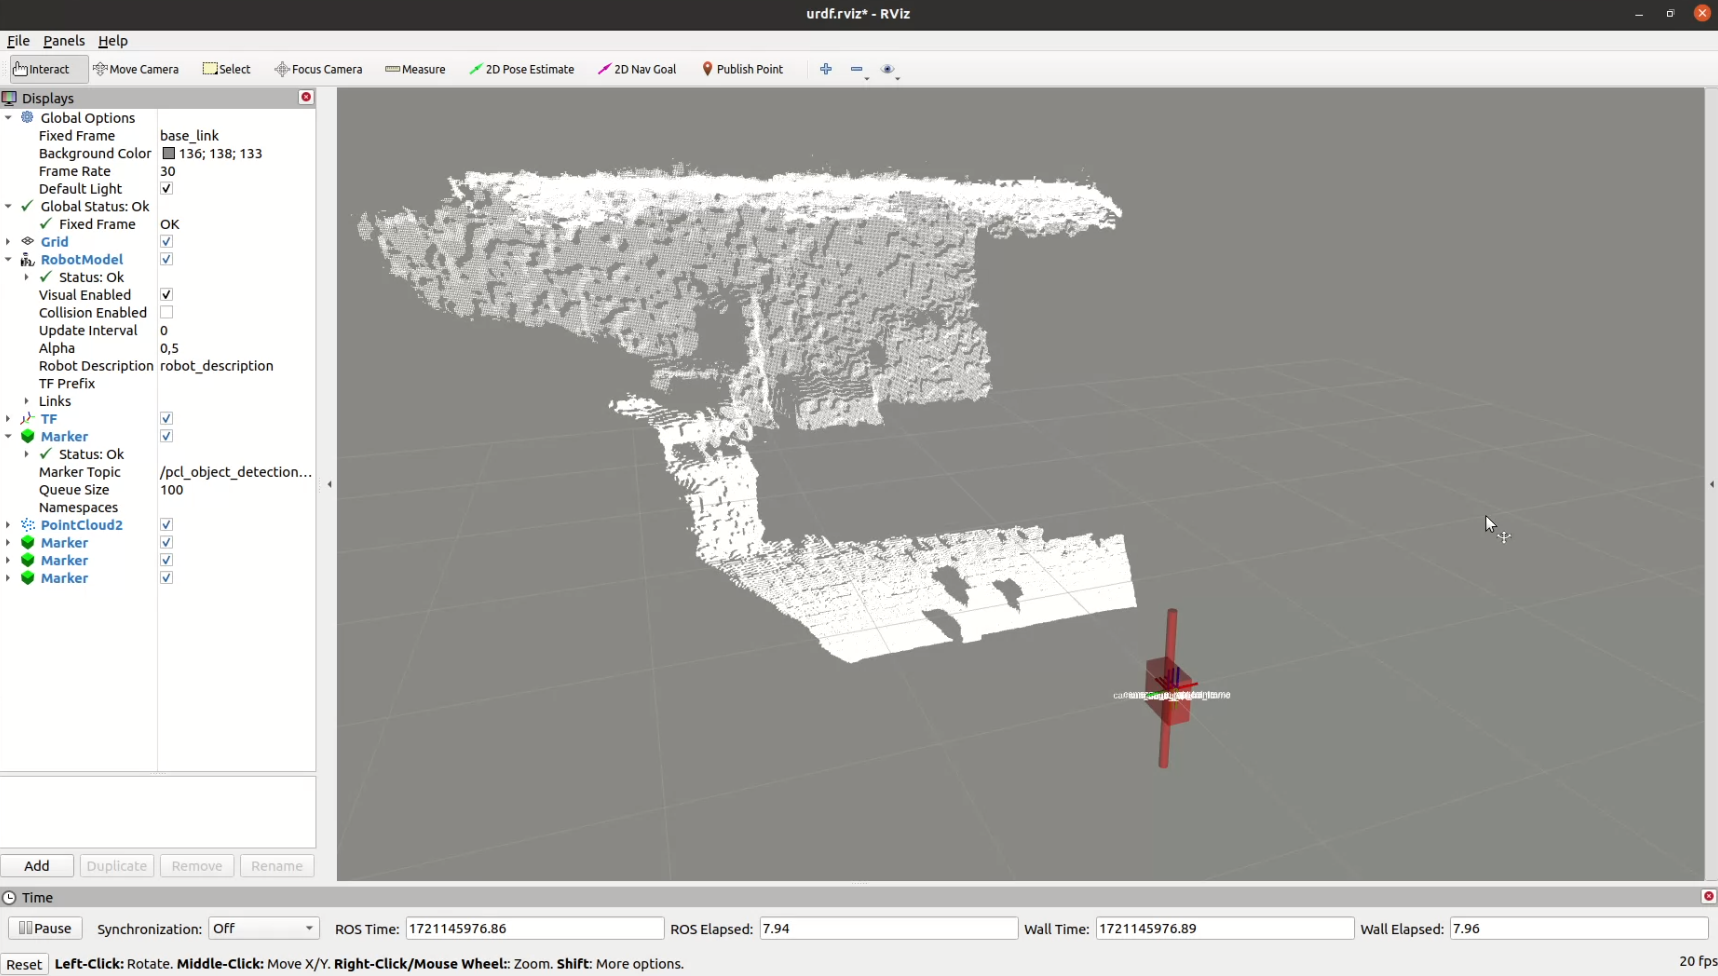
\includegraphics[width=0.5\linewidth]{rViz_1.png}
    \caption{Camera model and initial point cloud displayed in RViz}
    \label{fig:enter-label}
\end{figure}

The point cloud is processed using PCL: the data is filtered with VoxelGrid and used for plane segmentation. The remaining points, which are outside the plane, are divided into clusters.
Each cluster can eventually be considered as a detected object. We can specify parameters that limit the height and width to detect only a specific type of objects.\par
All clusters that meet the given conditions correspond to detected objects and their properties are published in the "pcl\_object\_detection/detected\_objects" message.\par


\begin{figure}[h]
    \centering
    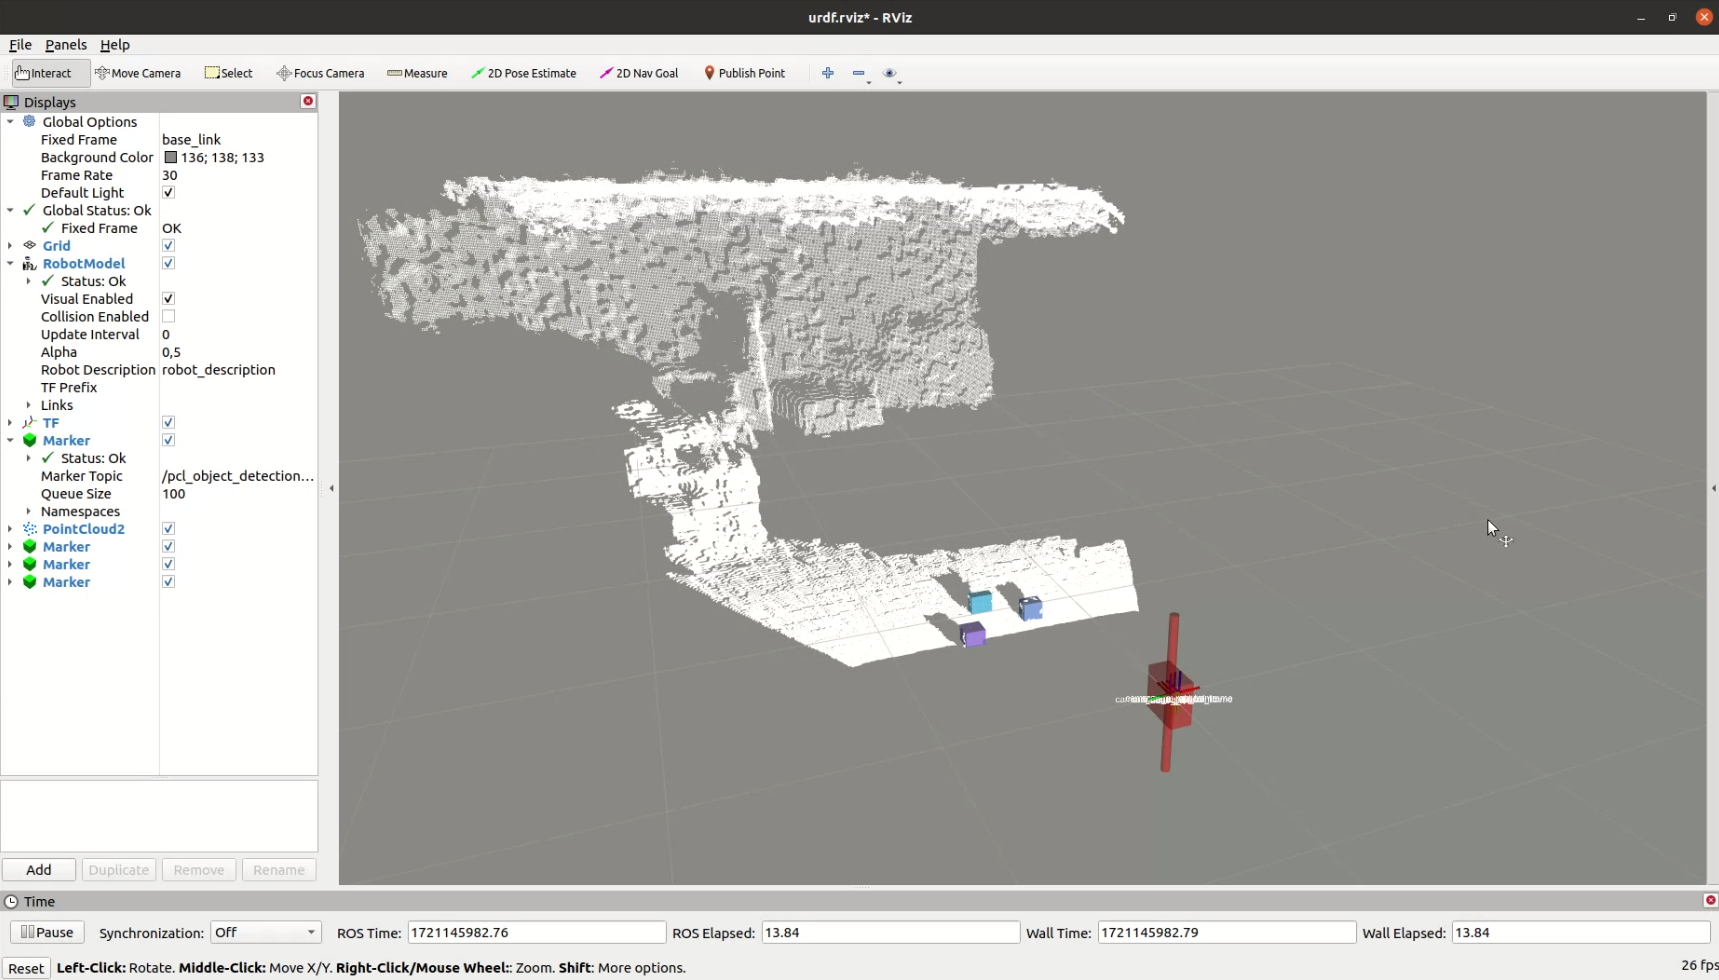
\includegraphics[width=0.5\linewidth]{rViz_2.png}
    \caption{Detected objects marked in blue}
    \label{fig:enter-label}
\end{figure}

\subsubsection{Detection in Experimental Environment}
Even if the scene with the objects was static, different objects were detected in consecutive depth clouds. The detection reliability decreased with the person moving in the scene.\par
I modified the original pcl\_object\_detection package from Shinsel Robots to improve the quality of object detection in my experimental environment. I also needed to implement a mechanism for switching between the ROS Astra driver and the Astra SDK to avoid issues with camera data accessibility.\par
The object size is limited to 20 cm and the object can be detected only when lying on the floor. Furthermore, a detection frame has been specified as a constraint for the object's location on the floor. An object outside the detection frame is ignored.\par
To ensure that the same objects are detected when the experiment is repeated in the same scene, I fixed the total number of objects and modified the program:\par
The received point clouds are processed one by one, with some objects detected in each cloud. \par
If the number of detected objects does not equal the total number, the result is ignored and processing continues with the next cloud.\par
Otherwise, the number of detected objects is correct, which usually means that only the correct objects have been detected. Their data is exposed in the "pcl\_object\_detection/detected\_objects" message. In addition, the message "object\_detection\_done" is published, which indicates that the ROS Astra driver is no longer needed.\par 
I added the "object\_detection\_done" subscriber to the ROS Astra driver. Once the message is received, the driver is shut down.\par

The package was also extended by code for displaying detected objects in RViz, marking them in blue and changing the color to red if the object was selected by the  pointing gesture.\par

\subsubsection{Gesture recognition}
The pointing\_gesture package implements methods for gesture recognition. It uses the Astra SDK to obtain body tracking information and allows several types of gesture recognition.\par
I modified the code from the astra\_body\_tracker package from Shinsels Robots. The package publishes body tracking information from the Astra SDK in the ROS topic, using messages from the body\_tracker\_msgs package.\par
The Astra SDK provides tools for skeleton recognition and body tracking. The tracked person is represented by a list of nineteen joints.\par
Corresponding body data includes the position and status of each joint, where status indicates the confidence level of the tracking with possible values of "NotTracked", "LowConfidence" and "Tracked".
The data also contains the current body tracking status, body orientation and hand pose.\par
The pointing\_gesture node is inactive during object detection. 
The "object\_detection\_done" message triggers the shutting down of the ROS Astra driver.\par
I added a subscriber for the "object\_detection\_done" topic to the pointing gesture node as well. Once the message is received, the node attempts to open the Astra data stream using the Astra SDK and repeats this until the ROS Astra device stream is completely terminated.\par
Then the data stream is available for the Astra SDK and we can start gesture recognition.\par 
The Astra SDK provides a list of tracked persons for each frame of the image data stream. For each tracked person, a check is made to evaluate whether he is performing the confirmation and pointing gestures.\par
The confirmation gesture is performed by raising the left hand. It is detected when the left hand joint is raised above the head joint.\par
I tried using the shoulder joint instead of the head joint. However, body tracking is not completely reliable and I observed many cases of false gesture detection. The shoulder joint has been often misidentified, while the head joint is usually identified correctly.\par
If a confirmation gesture is detected in a given frame, the right arm is checked for the pointing gesture, otherwise processing continues with the next frame.\par

\begin{figure}[h]
    \centering
    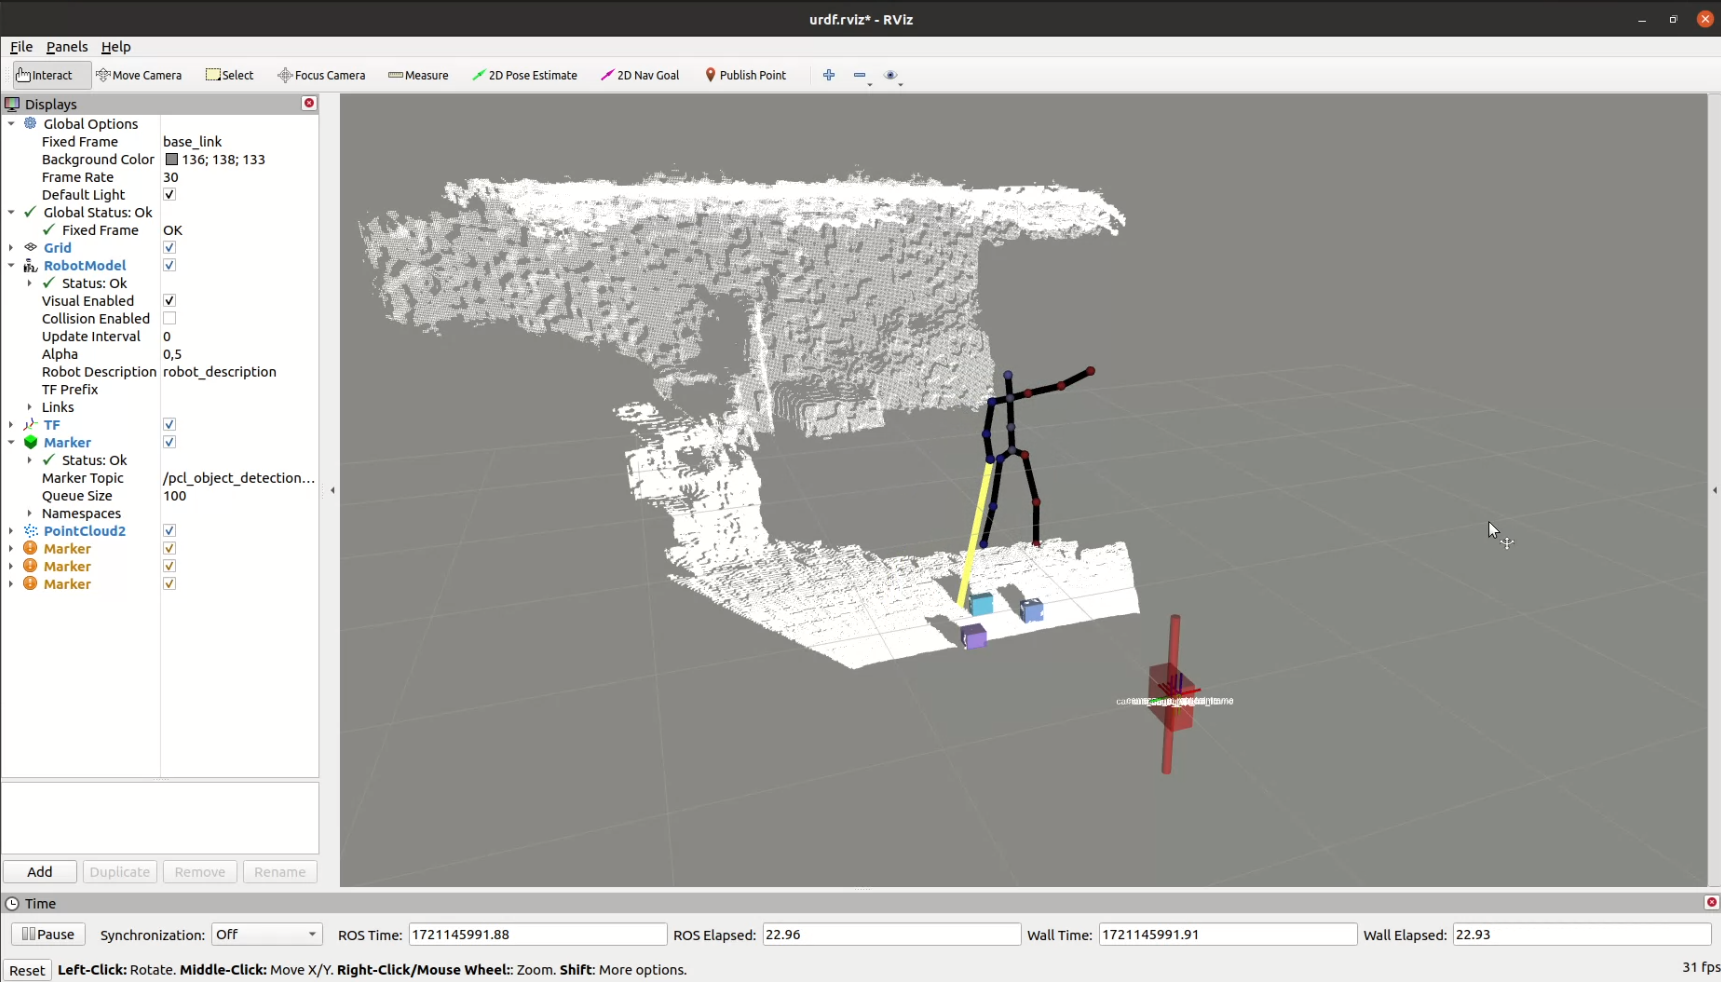
\includegraphics[width=0.5\linewidth]{rViz_3.png}
    \caption{Skeleton and pointing ray}
    \label{fig:enter-label}
\end{figure}

The pointing gesture is recognized by the position of the pair of joints corresponding to the selected pointing gesture type. The first joint of the pair determines the origin of the pointing ray. It is the upper joint when we consider the standard anatomical position.\par
The pointing gesture is detected when the first joint is positioned higher than the second.\par
The coordinates of the pointing ray intersection with the floor plane are computed and published in a ROS message.\par
The default option for the pointing gesture is the head-wrist type. The user may select a different option using a ROS message.\par


I have added RViz markers to display the skeleton of the tracked person and the pointing ray. When the first confirmed pointing gesture is detected and the intersection coordinates are published, the object closest to the intersection is selected and marked red in RViz. The distance between the intersection point and the object is logged.\par

\begin{figure}[h]
    \centering
    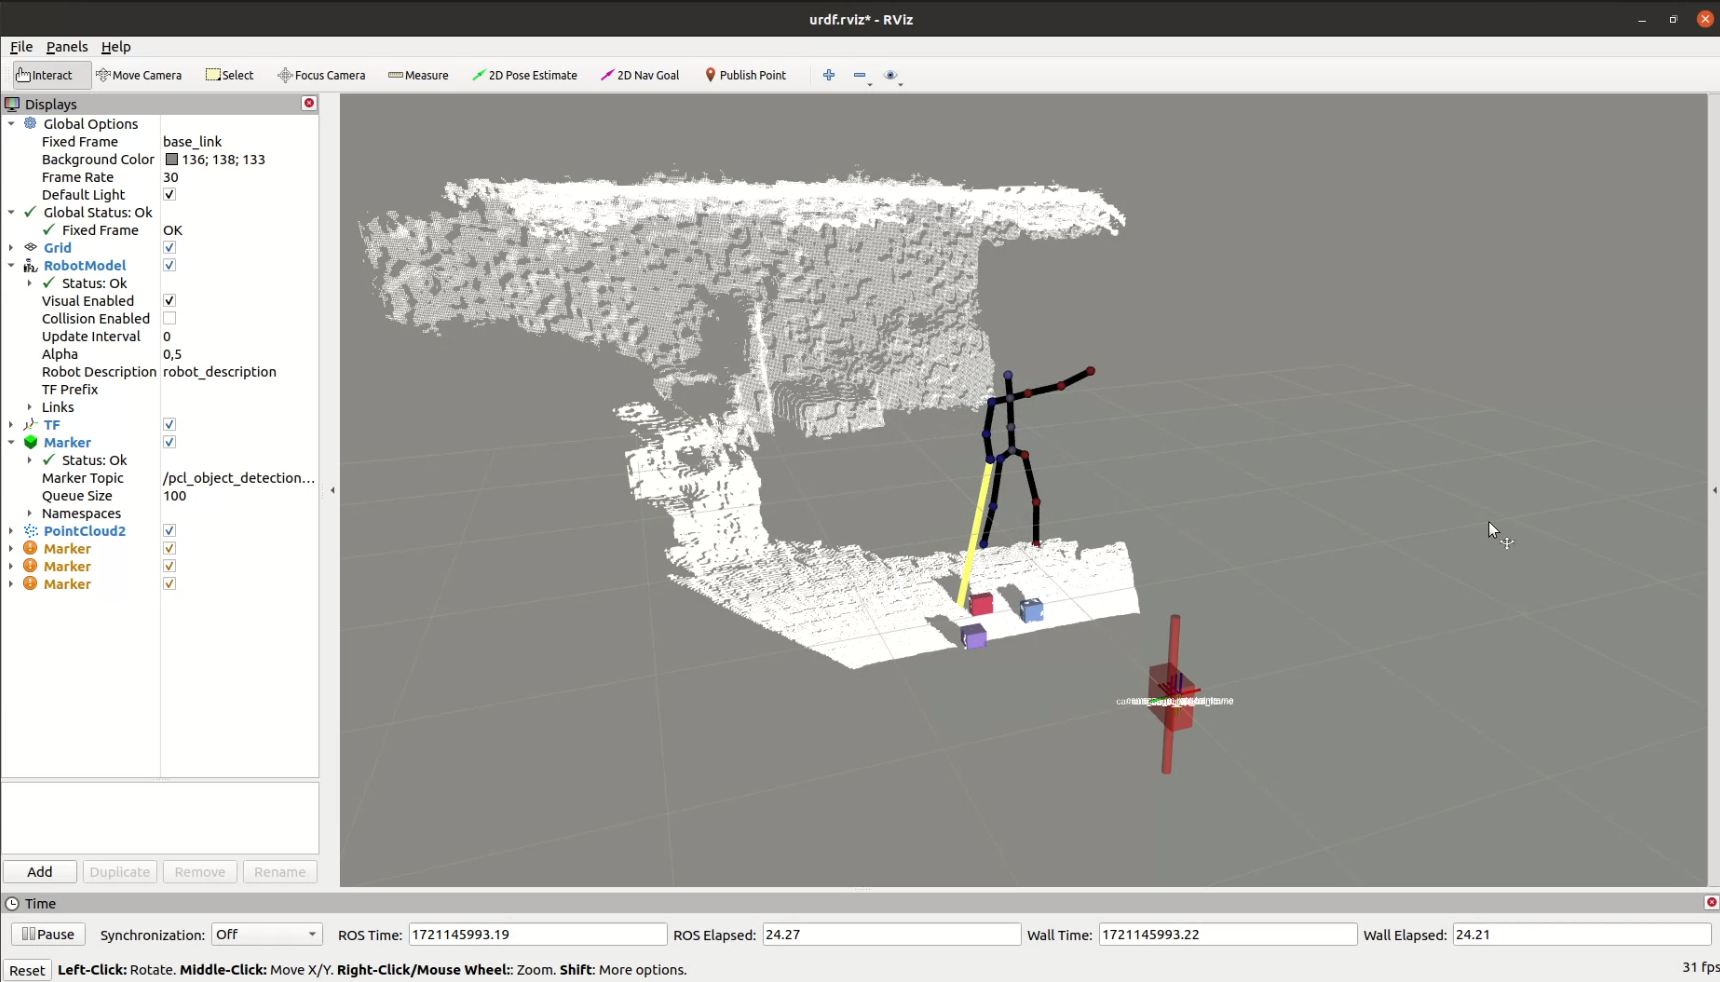
\includegraphics[width=0.5\linewidth]{rViz_4.png}
    \caption{Selected object marked in red}
    \label{fig:enter-label}
\end{figure}

The second detected pointing gesture specifies the target location.\par
Once the second confirmed pointing gesture is detected and the intersection is published, the data stream is closed.\par


\section{Mobile Robot Manipulator}

\subsection{Execution of Pick And Place Task}
I aimed to implement a Pick And Place task to test gesture based control with a real robot system and decided to use a mobile robotic manipulator for experiments.\par
Not all features for autonomous execution were fully implemented. I simplified the task because both navigation and object detection require detailed analysis and testing.\par
There is a restricted area in the robotics lab for the robot, with no obstacles except a few small objects on the floor. The surface is flat and even.\par
The robot knows its initial position and the coordinates of the camera. Once it receives the coordinates of the selected object and its target location, it navigates to the selected object and extends the robotic arm forward.\par
Since I have not completed the autonomous control of the robot arm, the gripper is not placed in the correct position and the robot needs help to pick up the object.\par
After five seconds, it closes the jaws of the gripper and can be sent to approximate target location where it releases the object.\par
The robot cannot handle unexpected events and will stop in a case of emergency.\par

\subsection{Autonomous Navigation}

\subsubsection{The Neobotix Mobile Robot}
The ROS Kinetic and Neobotix ROS packages have already been installed on the Neobotix mobile robot computer, as well as the ROS packages for navigation and motion control (ros-noetic-amcl, ros-noetic-map-server, ros-noetic-move-base).\par
I installed the ROS Noetic and packages from the Neobotix GitHub repository on my notebook. \par
The move\_base framework provides access to the ROS navigation stack and moves the robot to its goal destination. I implemented a SimpleActionClient that sends the goal state to move\_base.\par
The goal state includes the position and orientation of the robot. I needed to tune the parameters of the local Neobotix planner: the tolerance for the target orientation had to be increased because it was too strict for the robot.\par
I also modified robot's behaviour when unknown obstacles are detected. \par 
When the laser scanner detects an unknown obstacle in front of the robot, the robot creates a new motion plan and turns sideways to avoid a collision. This may lead to the detection of other new obstacles.\par

\begin{figure}[h]
    \centering
    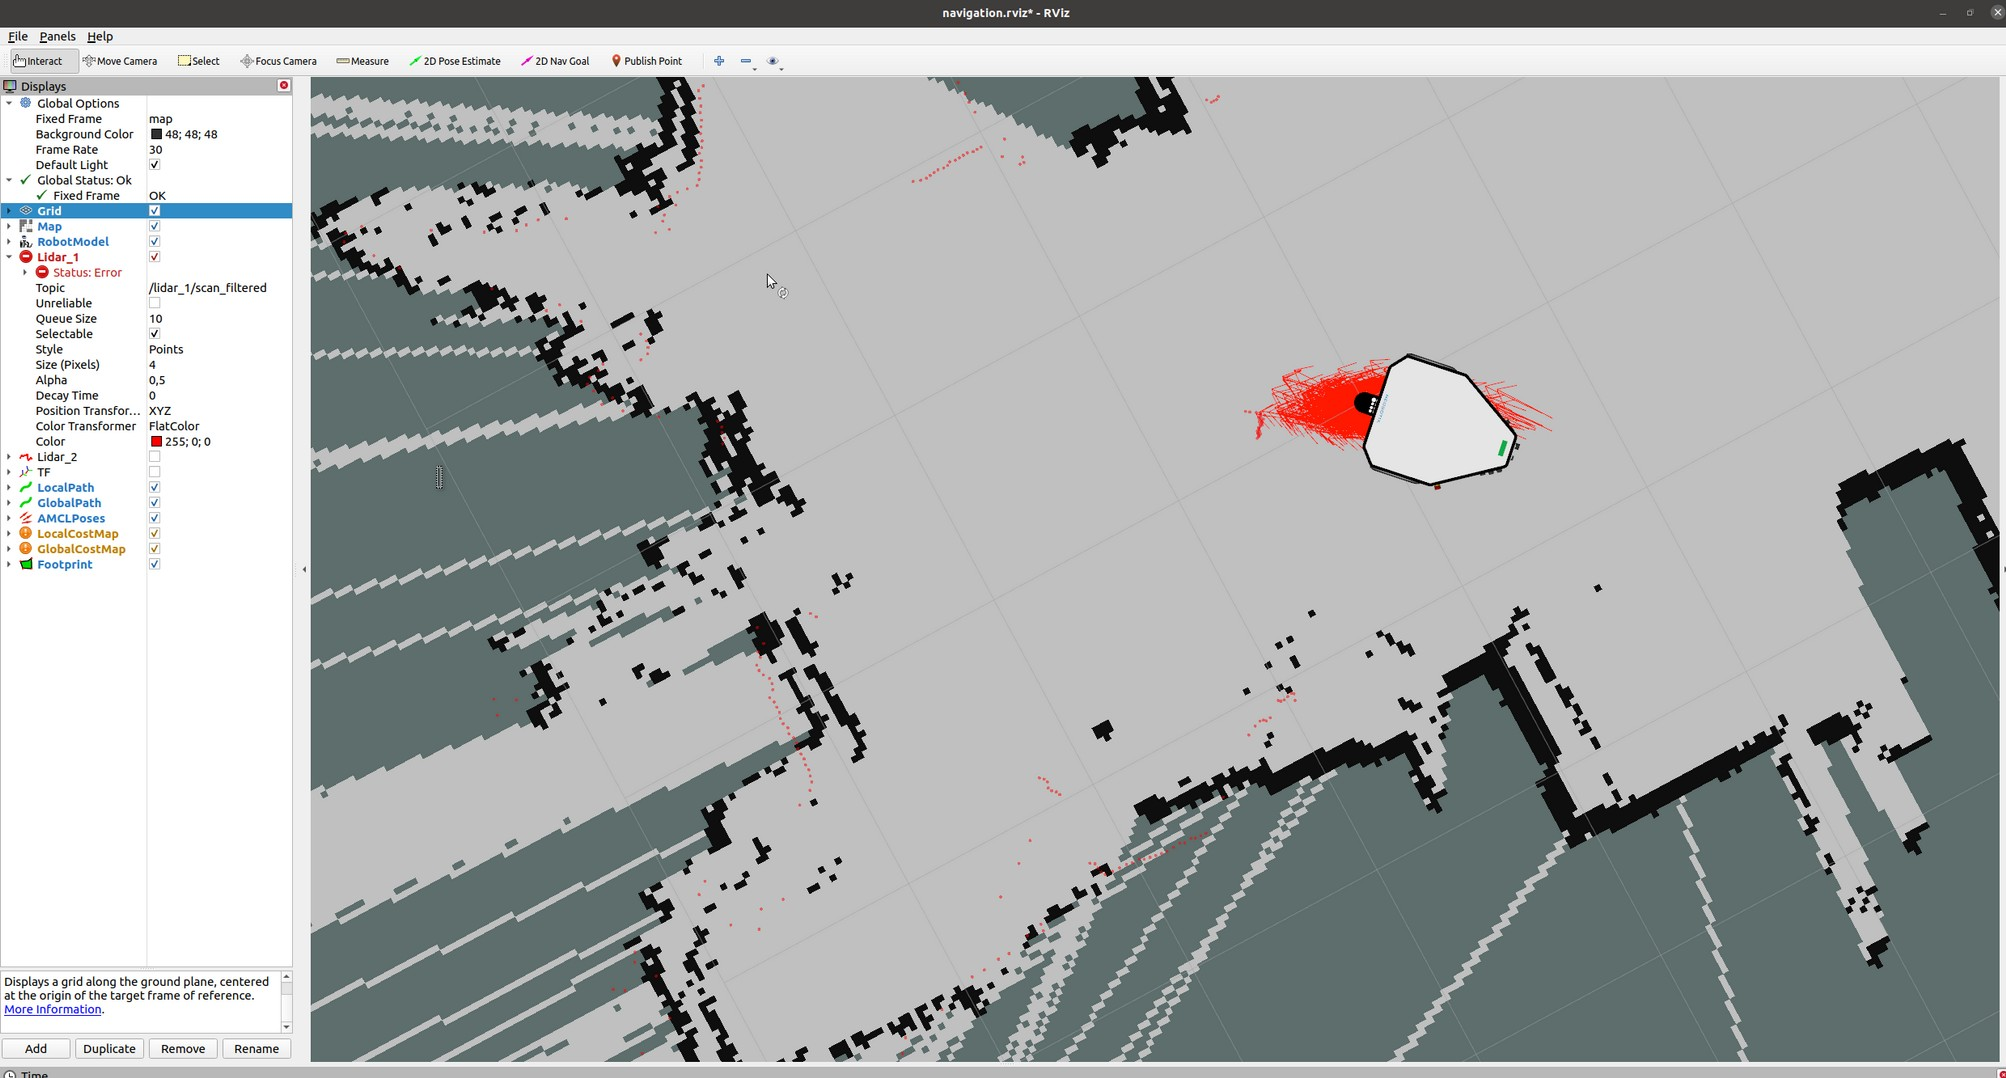
\includegraphics[width=0.5\linewidth]{rViz_navigation.png}
    \caption{Mobile robot manipulator in RViz}
    \label{fig:enter-label}
\end{figure}

By default, the robot will start to perform a recovery rotation when it cannot find any way out of its current position. I disabled this setting and increased the threshold for obstacle distance to enable the robot to approach the objects without unnecessary turning.\par

\subsubsection{Map of Environment}
The environment map can be created using the neo\_mp\_500 package, which provides tools for autonomous navigation. Simultaneous localization and mapping (SLAM) is performed using the gmapping algorithm.\par
I moved the robot around the lab using the remote control, checked the mapping process using rViz, and saved the map when it adequately represented the scene.\par

\begin{figure}[h]
    \centering
    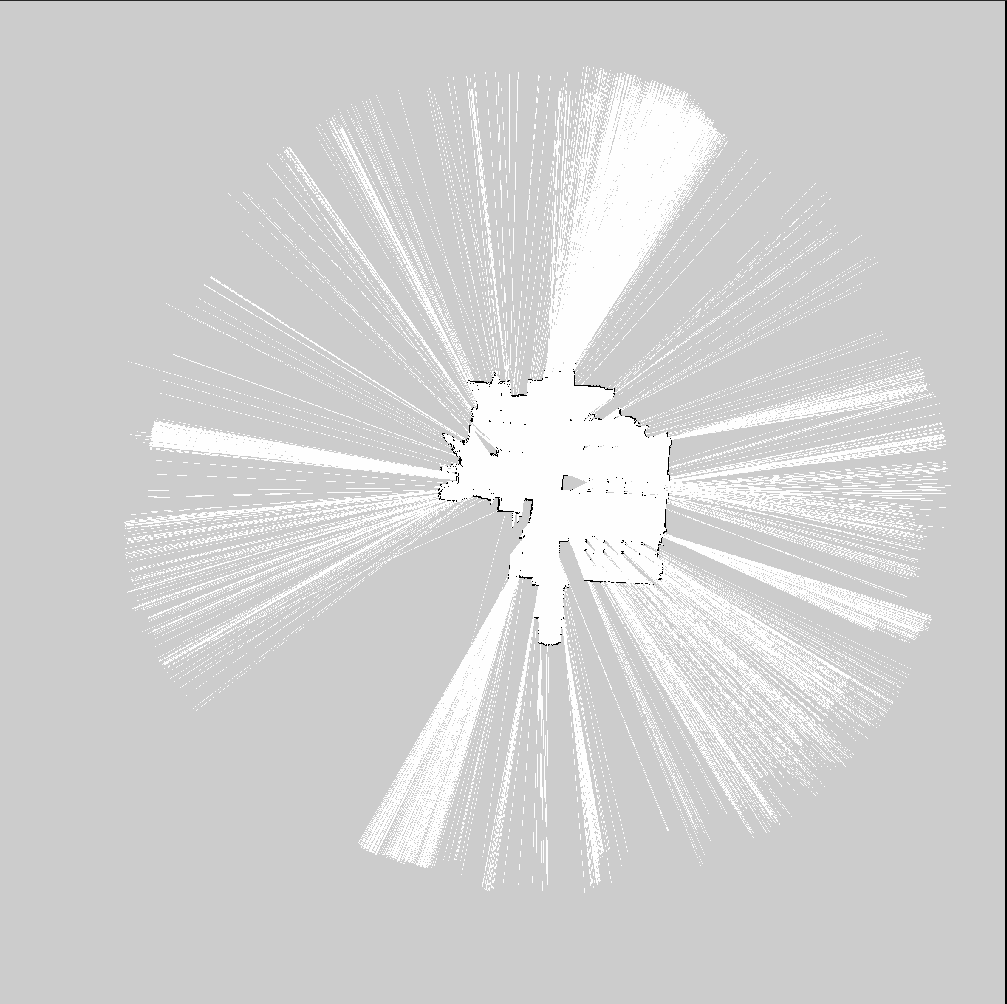
\includegraphics[width=0.5\linewidth]{map.png}
    \caption{Created map of environment}
    \label{fig:enter-label}
\end{figure}

\subsection{Object Manipulation}


\subsubsection{Universal Robots UR5 Manipulator}
TODO:\\
Universal Robots:\\
DashBoardServer, Polyscope, URP, ...\\

Packages:\\
Universal\_Robots\_ROS\_Driver
https://github.com/UniversalRobots/Universal\_Robots\_ROS\_Driver\\

Universal\_Robots\_Client\_Library\\
https://github.com/UniversalRobots/Universal\_Robots\_Client\_Library\\

ur5\_moveit\_config\\
https://github.com/ros-industrial/universal\_robot/tree/noetic-devel/ur5\_moveit\_config\\



\subsubsection{Mobile Manipulator URDF}
TODO:\\
URDF for Neobotix, UR5 and gripper.\\

\subsubsection{MoveIt Setup Assistant}
How to create config and set up arm positions.\\
How to set up arm limits.\\
Simulation in rViz.\\








